
\documentclass[12pt, a4paper]{article}
\usepackage{hyperref}
\hypersetup{
  colorlinks=true,
  linkcolor=blue,
  urlcolor=cyan,
}
\urlstyle{same}
\usepackage[utf8]{inputenc}
\usepackage{amsmath}
\usepackage{amsfonts}
\usepackage{amssymb}
\usepackage{graphicx}


\newtheorem{theorem}{Teorema.}
\newtheorem{lemma}[theorem]{Lema.}
\newtheorem{corollary}[theorem]{Corolario.}
\newtheorem{definition}[theorem]{Definici\'on:}
\newtheorem{example}[theorem]{Ejemplo:}
\newtheorem{problema}[theorem]{Problema:}
\newtheorem{remark}[theorem]{Observaci\'on:}

\usepackage{graphicx}
\usepackage[spanish]{babel}
%\usetheme{default}

\newcommand{\pp}{\mathbb{P}}
\newcommand{\zz}{\mathbb{Z}}
\newcommand{\rr}{\mathbb{R}}
\newcommand{\qq}{\mathbb{Q}}

\usepackage{tikz, tikz-3dplot}

\definecolor{cof}{RGB}{219,144,71}
\definecolor{pur}{RGB}{186,146,162}
\definecolor{greeo}{RGB}{91,173,69}
\definecolor{greet}{RGB}{52,111,72}

\date{}

\begin{document}
\title{Pr\'actico 1 TEOCOMP: Algoritmos codiciosos.}
\author{Mauricio Velasco}
\maketitle{}
\begin{enumerate} 
\item Implemente una clase \verb!Grafo_no_dirigido! que represente un grafo \verb!G! como lista de adyacencia. La clase debe recibir sólo el número de vértices del grafo e implementar las operaciones \verb!G.nueva_arista(i,j)! , \verb!G.nuevo_vertice()! y \verb!G.print()!.
\begin{enumerate}
\item Escriba el c\'odigo de su implementaci\'on.
\item Cu\'anta memoria (como funci\'on de $n$) requiere su clase para representar:
\begin{enumerate}
\item Un grafo completo $K_n$.
\item Un grafo bipartito completo $K_{n,n}$
\item Un ciclo de longitud $n$.
\item Un \'arbol con $n$ v\'ertices.
\end{enumerate} 
\end{enumerate}

\item({\it Árboles}) Recuerde que un {\bf árbol} es un grafo conexo y acíclico. Demuestre las siguientes afirmaciones:

\begin{enumerate}
\item Todo árbol con $n$ vértices tiene exáctamente $n-1$ aristas.
\item Las siguientes tres afirmaciones son equivalentes para todo grafo no dirigido $G$:
\begin{enumerate}
\item $G$ es un árbol.
\item $G$ es minimal conexo (es decir $G$ es conexo y quitarle cualquier arista lo vuelve disconexo).
\item $G$ es maximal acíclico (es decir $G$ no contiene ningún ciclo y adicionarle cualquier arista nueva hace aparecer al menos un ciclo en $G$).
\end{enumerate}
\end{enumerate} 


\item ({\it Cuántos árboles generadores tiene un grafo?}) El teorema de Birkhoff dice que el número de árboles generadores de un grafo no dirigido $G$ es igual al producto $(\lambda_1\dots\lambda_{n-1})/n$ donde los $\lambda_i$ denotan los valores propios diferentes de cero de la matriz $L=D-A$ donde $D$ es la matriz diagonal cuyas entradas son los grados de los vértices de $G$ y $A$ es la matriz de adyacencia de $G$. Realice los siguientes ejericios:
\begin{enumerate}
\item Si $G=K_4$ es el grafo completo de $4$ vértices, escriba la matriz $L$, calcule los valores propios y aplique la formula de Birkhoff. Dibuje todos los árboles generadores de $K_4$ y verifique que todo sea consistente.
\item Como es la matriz $L$ para el grafo $K_n$ completo con $n$ vértices?
\item Use el Teorema de Birkhoff y la matriz que calculo en la parte $(b)$ para demostrar que $K_n$ tiene $n^{n-2}$ árboles generadores posibles (para $n=50$ esto es más que el número estimado de átomos en el universo).
\item Escriba el código en Python de un algoritmo que calcule el número de árboles generadores de un grafo de la clase \verb!Grafo_no_dirigido! del punto $(1)$. Coméntelo adecuadamente y verifíquelo para grafos completos con la fórmula del numeral anterior. Cuál es el $n$ más grande al que puede llegar antes de que su computador sea incapaz de seguir?
\end{enumerate}
\item Sea $G$ un grafo no dirigido con pesos en las aristas. Encuentre un algoritmo para construir un árbol generador de {\bf máximo peso} para $G$ que pueda ejecutarse en tiempo $O((n+m)\log(n))$.
\newpage
\item ({\it El algoritmo de Prim.}) Sea $G$ el grafo con costos en las aristas del siguiente dibujo:
\begin{center}
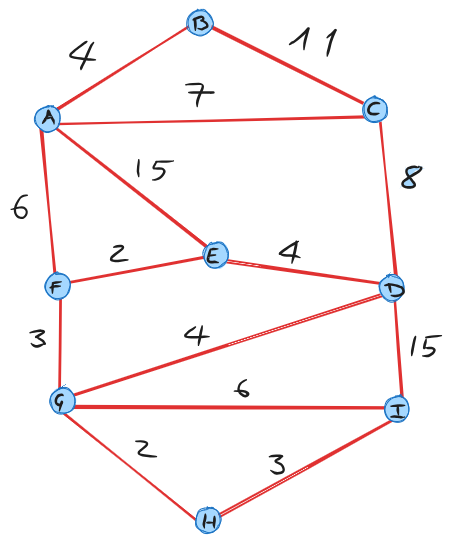
\includegraphics[scale=0.65]{MST.png}
\end{center}
\begin{enumerate}
\item Ejecute a mano el algoritmo de Prim para encontrar el mínimo árbol generador para $G$ con vértice inicial $A$. Escriba el vector $X$ que representa el orden en el que se incluyen los vértices y el vector $T$ de las aristas que lo constituyen. Dibuje el árbol generador obtenido.
\item Ejecute a mano el algoritmo de Kruskal para encontrar el mínimo árbol generador para $G$ con vértice inicial $A$.
\end{enumerate}

\item ({\it La propiedad de corte}) Sea $G$ un grafo no dirigido con costos en las aristas y suponga que los costos de todas las aristas son distintos. Un {\bf corte} en $G$ es una partición de los vértices en dos conjuntos disjuntos $A$ y $B$. Una arista {\bf cruza} el corte $(A,B)$ si tiene un vértice en $A$ y el otro en $B$. 
\begin{enumerate}
\item Demuestre la siguiente afirmación (llamada la propiedad de corte): Si una arista $e$ es la más barata que cruza un corte $(A,B)$ entonces $e$ pertenece a todo arbol generador de mínimo costo de $G$.
\item Utilice la propiedad del corte para dar una demostración alternativa de que el algoritmo de Prim produce un árbol generador de mínimo costo.
\end{enumerate}

\item ({\it Kruskal vs Prim}) El objetivo de este ejercicio es hacer una comparación empírica entre los algoritmos de Prim y Kruskal. 
\begin{enumerate}
\item Sea $G_n$ el grafo completo con $n$-vértices con pesos $1,2,3,\dots, \binom{n}{2}$ en las aristas.
\item Cuál es peso mínimo de un árbol generador en $G_n$? La respuesta debe depender de $n$. Demuestre la validez de su respuesta usando el algoritmo de Prim.
\item Implemente los algoritmos de Prim y Kruskal.
\item Escriba tablas que midan el tiempo de ejecución y la memoria utilizada para encontrar el MST para los grafos $G_n$ para diferentes valores de $n$ (cuál es el máximo $n$ en el que su algoritmo funciona?).
\item Escriba un párrafo que resuma sus conclusiones: Es alguno de los dos mejor que el otro en algún aspecto? Argumente su respuesta.
\end{enumerate}

\item ({\it Kruskal bueno}) Investigue los siguientes puntos:
\begin{enumerate}
\item Describa de manera precisa la estructura de datos \verb!union find!.
\item Escriba el código en python de una implementación eficiente del algoritmo de Kruskal usando \verb!union find!.
\item Cálcule el tiempo requerido por su implementación argumentando la validez de su respuesta de manera precisa.
\end{enumerate}


\end{enumerate}
\end{document}

\item Visitamos todos los v\'ertices del grafo no dirigido con $V=\{1,\dots, 7\}$ y con aristas $E$ determinadas por $(1,2), (1,3)$ $(3,7), (3,6), (2,4)$ y $(2,5)$ iniciando en el v\'ertice $(2)$.
\begin{enumerate}
\item Escriba la lista de v\'ertices en el orden en el que los visitar\'iamos en BFS.
\item Hay otro orden posible adicional al que escribi\'o en el numeral anterior?
\item Cu\'antos \'ordenes posibles hay? Escr\'ibalos todos.
\item Generalizado el ejemplo anterior, cu\'antos \'ordenes BFS cree que hay para recorrer un \'arbol binario con $\ell$ niveles?.
\end{enumerate}

\item Sea $A$ la matriz de adyacencia de un grafo $G$. Demuestre que para cualquier entero positivo $k$ y para cualquier par de v\'ertices $i,j$ se tiene que $(A^{k})_{ij}$ es igual al n\'umero de caminos desde $i$ hasta $j$ de longitud $k$.

\item{Recuerde que un \'arbol es, por definici\'on, un grafo conexo y sin ciclos. Demuestre las siguientes afirmaciones:
\begin{enumerate}
\item Si $G$ es un grafo con $n$ v\'ertices y $m$ aristas entonces $m=O(n^2)$.
\item Todo \'arbol con $n$ v\'ertices tiene $n-1$ aristas.
\item Concluya que si $G$ es un grafo conexo con $m$ v\'ertices entonces $m=\Omega(n)$ y $m=O(n^2)$.
\end{enumerate}
}


\item Implemente una funci\'on que reciba un \texttt{Grafo} $H$ y el \'indice de un v\'ertice de $H$ y retorne un árbol breadth-first-search $T$ para $H$. El árbol $T$ debe ser una instancia de la clase \texttt{Grafo} del problema $(1)$.



\begin{enumerate}
\item Escriba el c\'odigo de su implementaci\'on.
\item Utilice su implementaci\'on en el grafo del siguiente dibujo iniciando en el v\'ertice $D$ 
\begin{center}
\includegraphics[scale=0.5]{grafo_1.png}
\end{center}
y dibuje el \'arbol $T$ obtenido.
\end{enumerate}


\end{enumerate}


\end{document}



